\begin{center}	
\textbf{BOLETÍN DE EJERCICIOS 4}
\end{center}

\vspace{2cm}

\begin{enumerate}[\textbf{Ejercicio} 1.]

    %--------------------Ejercicio 1.	
    \item Para el país elegido por el grupo y para España realizar con los datos de los últimos 20 años en total y por subperiodos  tal y como se presento en clase la Contabilidad del Crecimiento.\\\\

    \begin{table}[htbp]
      \centering
      \caption{Contabilidad del crecimiento Española}
      \scalebox{0.5}{
      \begin{tabular}{cccccccc}
	\toprule
	\midrule
	&&&\multicolumn{5}{c}{Fuente de crecimiento}\\
	\cmidrule{4-8}
	& Crecimiento de la producción&&Capital&&trabajo&&Produc. Total de los factores\\ 
	    Años&$\triangle Y/Y$&=& $\alpha \triangle K/K$ &+& $(1-\alpha)\triangle L/L$ &+& $\triangle A/A$ \\
	\midrule
	    \multicolumn{8}{c}{Aumento porcentual medio anual}\\\\
		2002-2012&1.06&&-0.71&&0.19&&1.58\\
		2013-2022&1.56&&1.26&&0.83&&-0.53\\
		2002-2022&1.16&&0.08&&0.41&&0.66\\
	\bottomrule
	\end{tabular}%
	}
      \label{tab:addlabel}%
      \begin{center}
      \tiny Fuente: Celcdata.
      \end{center}
    \end{table}


    \begin{table}[htbp]
      \centering
      \caption{Contabilidad del crecimiento Alemán}
      \scalebox{0.5}{
      \begin{tabular}{cccccccc}
	\toprule
	\midrule
	&&&\multicolumn{5}{c}{Fuente de crecimiento}\\
	\cmidrule{4-8}
	& Crecimiento de la producción&&Capital&&trabajo&&Produc. Total de los factores\\ 
	    Años& $\triangle Y/Y$ &=& $\alpha \triangle K/K$ &+& $(1-\alpha)\triangle L/L$ &+& $\triangle A/A$ \\
	\midrule
	    \multicolumn{8}{c}{Aumento porcentual medio anual}\\\\
		2002-2012&1.14&&0.60&&0.33&&0.21\\
		2013-2022&1.24&&0.97&&0.36&&-0.08\\
		2002-2022&1.15&&0.69&&0.35&&0.10\\
	\bottomrule
	\end{tabular}%
	}
      \label{tab:addlabel}%
      \begin{center}
      \tiny Fuente: Celcdata.
      \end{center}
    \end{table}

    %--------------------Ejercicio 2.
    \item Para el país elegido y para España, con los datos actualizados intentar replicar lo presentado en las siguientes diapositivas que se presentaron en clase.\\\\

    \begin{center}
	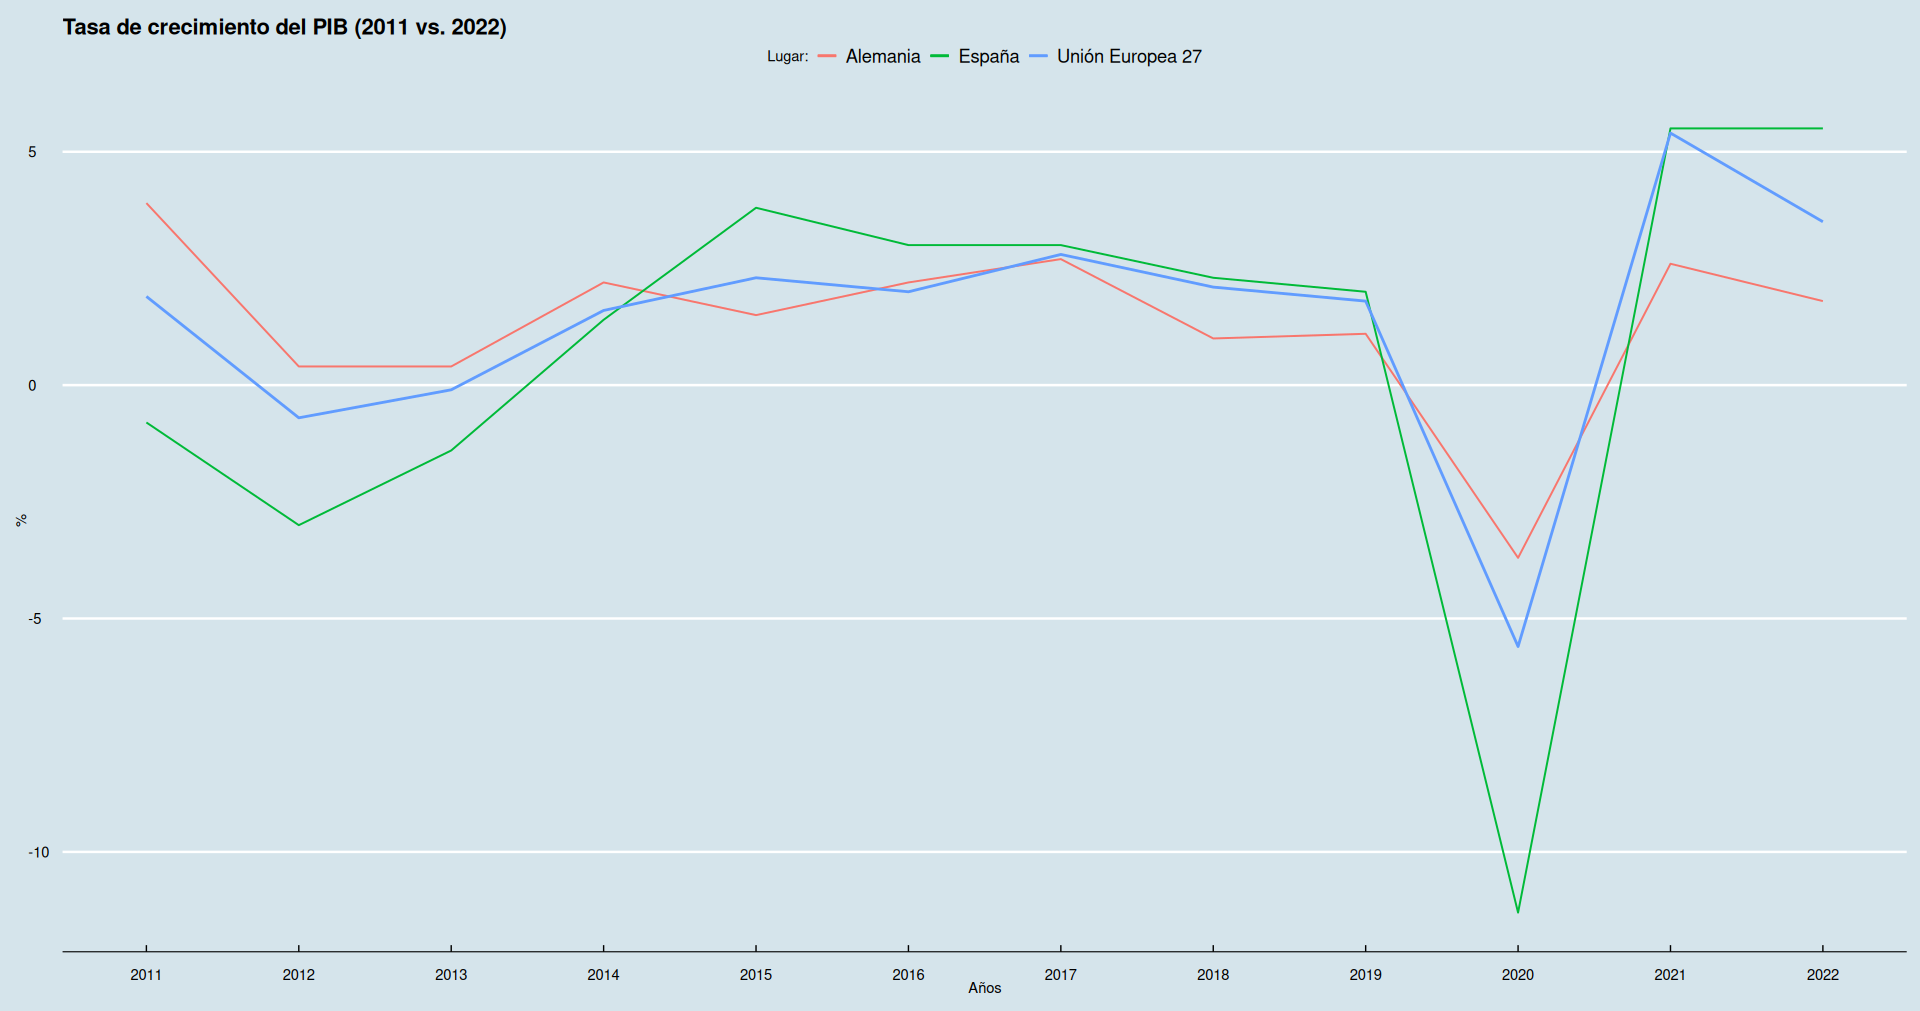
\includegraphics[scale=.29]{image/b4ej1_1.png}
    \end{center}

    Sin una notable diferencial de crecimiento con la UE-27 y los países estudiados, pero explicado en buena parte por la población. Por ello, ha sido insuficiente para alcanzar la plena convergencia.

\end{enumerate}
